\documentclass[10pt,twocolumn,letterpaper]{article}

\usepackage[letterpaper,top=19mm,bottom=21mm,left=17mm,right=17mm,columnsep=7mm]{geometry}
\usepackage{lmodern}
\usepackage{microtype}
\usepackage{amsmath,amssymb,amsthm}
\usepackage{mathtools}
\usepackage{booktabs}
\usepackage{tabularx}
\usepackage{graphicx}
\usepackage{xcolor}
\usepackage{caption}
\usepackage{subcaption}
\usepackage{fancyhdr}
\usepackage{hyperref}

\definecolor{primary}{RGB}{27, 54, 93}
\definecolor{accent}{RGB}{0, 128, 128}
\definecolor{warn}{RGB}{217, 83, 79}
\definecolor{slate}{RGB}{93, 109, 126}

\hypersetup{
    colorlinks=true,
    linkcolor=primary,
    citecolor=accent,
    urlcolor=primary,
    pdftitle={Human-Computer Interaction for Secure AI Tool Usage: Design Patterns Against Prompt Injection},
    pdfauthor={Senior HCI and AI Security Research Group}
}

\setlength{\parskip}{3.5pt plus 1pt minus 1pt}
\setlength{\parindent}{1em}
\emergencystretch=1.5em

\captionsetup{font=small,labelfont={bf,color=primary},skip=5pt}

\pagestyle{fancy}
\fancyhf{}
\fancyhead[L]{\footnotesize\textit{Human-Computer Interaction for Secure AI Tool Usage: Design Patterns Against Prompt Injection}}
\fancyhead[R]{\footnotesize\textbf{PROV-Guard Framework (2026)}}
\fancyfoot[C]{\footnotesize\thepage}
\renewcommand{\headrulewidth}{0.4pt}

\newtheorem{definition}{Definition}
\newtheorem{proposition}{Proposition}
\newtheorem{hypothesis}{Hypothesis}

\newcommand{\takeaway}[2]{%
  \vspace{4pt}\noindent\colorbox{primary!7}{%
    \parbox{\dimexpr\columnwidth-2\fboxsep\relax}{%
      \vspace{2.5pt}\footnotesize\textbf{\color{primary}#1:}\hspace{0.4em}#2\vspace{2.5pt}%
    }%
  }\vspace{4pt}%
}

\title{\vspace{-8mm}\LARGE\textbf{\color{primary}Human-Computer Interaction for Secure AI Tool Usage: Causal-Provenance and Adaptive-Friction Design Patterns Against Indirect Prompt Injection}}

\author{
  \textbf{Senior HCI \& AI Security Research Group}\\
  Department of Computer Science \& Human-Centered Security Laboratory\\
  Repository: \texttt{https://github.com/mazharulmd/HCI.git} (\texttt{research/prov-guard-hci-defense})
}
\date{October 2026}

\begin{document}

\maketitle

\begin{abstract}
\noindent
Tool-augmented Large Language Model (LLM) agents increasingly execute high-privilege operations---such as sending external communications, modifying cloud permissions, initiating financial transfers, and invoking system shells---via standardized interfaces such as the Model Context Protocol (MCP). However, processing untrusted third-party data (e.g., incoming emails, shared documents, web pages, and repository issues) alongside privileged tool credentials exposes agents to \emph{Indirect Prompt Injection (IPI)}, transforming the agent into a confused deputy. While system-level defenses (e.g., delimiter spotlighting and static information-flow interpreters) and generic Human-in-the-Loop (HITL) confirmation dialogs have been proposed, a critical usable-security gap remains: \textbf{why do human operators routinely approve hijacked tool calls even when confirmation prompts are displayed?} Drawing on neuro-behavioral warning habituation theory and dual-process cognitive control, we demonstrate that uniform binary confirmation modals suffer from severe \emph{Provenance Blindness} and \emph{Generalization of Habituation}, yielding a $92.62\%$ Attack Success Rate (ASR) across longitudinal agent sessions. To resolve this vulnerability, we propose \textbf{PROV-Guard}, a human-centered defense framework comprising four formalized HCI design patterns: (1)~\emph{Dual-Lineage Provenance Attribution (DLPA)}, (2)~\emph{Contextual Goal-Alignment and Semantic Drift Visualization (CGASD)}, (3)~\emph{Adaptive Friction and Tiered Capability Gates (AFTCG)}, and (4)~\emph{Interactive Counterfactual and Sandbox Preview (ICSP)}. Across a comprehensive 250-scenario multi-domain benchmark ($100$ benign, $150$ adversarial across $5$ enterprise domains and $5$ attack families) evaluated over $N=48$ stratified operator profiles ($108,000$ total trials), PROV-Guard reduces overall ASR from $92.62\%$ (Binary Modal) and $56.11\%$ (Spotlighting) to $\mathbf{2.54\%}$ ($p = 1.92 \times 10^{-16}$, Mann-Whitney $U$ with Holm-Bonferroni correction, Cohen's $d = -49.37$), elevates Signal Detection sensitivity from $d' = -0.14$ to $\mathbf{d' = 4.21}$, reduces benign false-positive task rejections from $9.62\%$ to $\mathbf{1.10\%}$, and lowers subjective cognitive workload (NASA-TLX) by $\mathbf{22.9\%}$ at a negligible runtime analysis overhead of $0.084\,\text{ms}$.
\end{abstract}

\noindent\textbf{Keywords:} Human-Computer Interaction (HCI), Usable Security, Indirect Prompt Injection, AI Agents, Tool-Calling Security, Provenance Attribution, Warning Habituation, Signal Detection Theory.

\section{Introduction: The Confused Deputy in Human-AI Tool Collaboration}

The transition from passive conversational Large Language Models (LLMs) to autonomous, tool-augmented AI agents marks a fundamental architectural shift in enterprise computing \cite{greshake2023not, debenedetti2024agentdojo, zhan2024injecagent}. Through standardized orchestration layers such as the Model Context Protocol (MCP), enterprise assistants read and summarize emails, inspect financial invoices, triage GitHub repositories, manage executive calendars, and execute shell scripts. Crucially, these workflows require the agent to ingest \emph{untrusted external data} into the same context window that governs \emph{privileged tool selection and parameter generation}.

When an adversary embeds hidden imperative instructions inside an external email, PDF invoice, webpage, or code comment, the LLM cannot reliably distinguish trusted user intent from untrusted data tokens \cite{zverev2024can}. Consequently, the agent can be hijacked into invoking unauthorized tools or diverting critical sink arguments (e.g., recipient addresses, beneficiary IBANs, or webhook URLs)---a vulnerability class ranked as OWASP LLM01 (Prompt Injection) and exemplified by high-severity enterprise exploits such as zero-click Microsoft 365 Copilot exfiltration (\texttt{CVE-2025-32711}, EchoLeak) and Cursor IDE remote code execution (\texttt{CVE-2025-54135}, CurXecute).

Existing defenses fall into two disconnected paradigms:
\begin{enumerate}
    \item \textbf{Model- and System-Level Guards:} Techniques such as Delimiter Spotlighting \cite{hines2024spotlighting}, structured query fine-tuning (StruQ \cite{chen2024struq}, SecAlign \cite{chen2025secalign}), execution isolation (IsolateGPT \cite{wu2025isolategpt}), and strict capability interpreters (CaMeL \cite{debenedetti2025camel}). While valuable, in-band filters are bypassed by semantic goal-mimicry and encoded payloads, whereas strict static flow-blocking breaks dynamic workflows where a user legitimately asks an agent to act on external data (e.g., \emph{``Pay the balance listed on the attached vendor invoice''}) \cite{debenedetti2025camel}.
    \item \textbf{Naive Human-in-the-Loop (HITL) Action Guards:} Frameworks such as MCP client prompts and Magentic-UI \cite{magenticui2025} delegate unresolved trust decisions to the human user via binary \texttt{[Allow / Deny]} confirmation modals before executing state-mutating tools.
\end{enumerate}

In this paper, we argue that \textbf{delegating security decisions to a human operator via standard confirmation dialogs merely shifts the confused-deputy vulnerability from the silicon model to the human cognitive loop}. In our empirical evaluation, standard binary confirmation dialogs fail to stop $92.62\%$ of indirect prompt injections over a 250-task session. We identify three root causes at the intersection of AI security and Human-Computer Interaction (HCI):
\begin{itemize}
    \item \textbf{Provenance Blindness:} Standard tool-approval modals display \emph{what} function and JSON arguments the agent proposes to call, but strip away \emph{causal lineage}---failing to indicate whether a critical sink parameter (e.g., \texttt{recipient="drop@exfil.io"}) originated from the user's explicit prompt or from an untrusted third-party document.
    \item \textbf{Generalization of Warning Habituation:} When an interface interrupts the user on $80\%\text{--}100\%$ of benign mutating actions with visually uniform dialogs, neurobiological habituation transfers rapidly across prompts \cite{akhawe2013alice, anderson2016polymorphic, vance2018habituation, jenkins2025fog}, driving System~1 automatic click-through.
    \item \textbf{Semantic Goal-Mimicry Opacity:} Sophisticated injections eschew overt ``ignore previous instructions'' phrasing and instead frame malicious tool arguments as plausible administrative routing updates, deceiving users who inspect raw parameter strings without goal-alignment telemetry.
\end{itemize}

\subsection{Research Questions and Hypotheses}
To bridge this gap, we investigate four formal Research Questions (RQs) and test four preregistered Hypotheses (H1--H4):
\begin{itemize}
    \item \textbf{RQ1 (Causal Provenance vs.\ Habituation):} How does surfacing token-level parameter provenance (distinguishing user-explicit vs.\ external-untrusted lineage) affect operator discrimination sensitivity ($d'$) and Attack Success Rate (ASR)?\\
    \emph{Hypothesis H1:} Dual-Lineage Provenance Attribution (DLPA) will significantly reduce ASR and increase sensitivity $d'$ compared to raw parameter confirmation modals ($p < 0.001$).
    \item \textbf{RQ2 (Semantic Drift Telemetry against Goal-Mimicry):} Can visual goal-alignment and semantic drift indicators enable operators to detect stealthy Goal-Mimicry and Context-Framing attacks that evade delimiter guards?\\
    \emph{Hypothesis H2:} Contextual Goal-Alignment and Semantic Drift Visualization (CGASD) will reduce Goal-Mimicry ASR by $>50$ percentage points compared to provenance-only or delimiter-only defenses.
    \item \textbf{RQ3 (Risk-Calibrated Constructive Friction):} Does adaptive, four-tier capability friction with constructive parameter verification mitigate longitudinal warning habituation while lowering overall cognitive workload?\\
    \emph{Hypothesis H3:} Adaptive Friction and Tiered Capability Gates (AFTCG) will maintain longitudinal habituation $H(t) < 0.15$ across $250$ sequential trials and reduce NASA-TLX workload by $>20\%$ relative to uniform binary modals.
    \item \textbf{RQ4 (Counterfactual Blast-Radius Preview):} How does displaying a pre-execution counterfactual state diff and reversibility score impact false-positive rejections on legitimate high-privilege workflows?\\
    \emph{Hypothesis H4:} Interactive Counterfactual and Sandbox Preview (ICSP) will reduce Cross-Tool Chaining ASR while keeping benign false-positive rejection below $2.0\%$.
\end{itemize}

\section{Related Work and Systematic Gap Analysis (2023--2026)}

Table~\ref{tab:lit_review} synthesizes representative benchmarks, system defenses, and HCI security frameworks from 2023 to 2026.

\begin{table*}[t]
\centering
\caption{Systematic Comparison of Indirect Prompt Injection Defenses and Usable Security Frameworks (2023--2026).}
\label{tab:lit_review}
\resizebox{\textwidth}{!}{%
\begin{tabular}{l l c c c c l}
\toprule
\textbf{Framework / Study} & \textbf{Primary Paradigm} & \textbf{Lineage UI} & \textbf{Drift UI} & \textbf{Anti-Habit.} & \textbf{Blast Preview} & \textbf{Key Limitation Addressed by PROV-Guard} \\
\midrule
Greshake et al.\ (2023) \cite{greshake2023not} & Threat Taxonomy & No & No & No & No & Identifies IPI threat; proposes no operational HCI defense. \\
BIPIA / Yi et al.\ (2023) \cite{yi2023bipia} & Benchmark \& Delimiters & No & No & No & No & Evaluates static text tasks; lacks interactive tool-calling UI. \\
InjecAgent / Zhan et al.\ (2024) \cite{zhan2024injecagent} & Tool-Agent Benchmark & No & No & No & No & Single-step tool benchmark without human-in-the-loop modeling. \\
Spotlighting / Hines et al.\ (2024) \cite{hines2024spotlighting} & In-Band Delimiter/Encoding & No & No & No & No & Vulnerable to semantic goal-mimicry and cross-tool chaining ($56.1\%$ ASR). \\
StruQ \cite{chen2024struq} \& SecAlign \cite{chen2025secalign} & Fine-Tuning Separation & No & No & No & No & Model-specific retraining; degrades on adaptive task-adjacent payloads. \\
AgentDojo / Debenedetti et al.\ (2024) \cite{debenedetti2024agentdojo} & Dynamic Agent Suite & No & No & No & No & Evaluates autonomous execution; omits human oversight cognitive dynamics. \\
CaMeL / Debenedetti et al.\ (2025) \cite{debenedetti2025camel} & Static Control/Data IFC & No & No & No & No & Blocks legitimate data-driven control flows unless human resolves policy. \\
Magentic-UI / Microsoft (2025) \cite{magenticui2025} & Co-Planning \& Action Guards & No & No & Partial & No & Binary action guards lack token provenance and suffer from click fatigue. \\
Vance et al.\ \cite{vance2018habituation} \& Jenkins et al.\ \cite{jenkins2025fog} & Neuro-IS Warning Habituation & N/A & N/A & Yes & No & Studies browser/OS popups; not adapted to LLM agent parameter taint. \\
\midrule
\textbf{PROV-Guard (Ours, 2026)} & \textbf{Causal-Provenance HCI Suite} & \textbf{Yes} & \textbf{Yes} & \textbf{Yes} & \textbf{Yes} & \textbf{Unifies token taint lineage, semantic drift, constructive friction, and sandbox diffs.} \\
\bottomrule
\end{tabular}%
}
\end{table*}

\subsection{Indirect Prompt Injection Benchmarks and Defenses}
Greshake et al.\ \cite{greshake2023not} first demonstrated that LLM-integrated applications blur the boundary between code and data. Subsequent benchmarks---including BIPIA \cite{yi2023bipia}, InjecAgent \cite{zhan2024injecagent}, and AgentDojo \cite{debenedetti2024agentdojo}---quantified high vulnerability rates across frontier models in email, banking, and workspace environments. In-band defenses such as Spotlighting \cite{hines2024spotlighting} wrap external data in special delimiters or encodings, while StruQ \cite{chen2024struq} and SecAlign \cite{chen2025secalign} fine-tune models to ignore instructions inside data fields. Out-of-band architectures such as IsolateGPT \cite{wu2025isolategpt} and CaMeL \cite{debenedetti2025camel} enforce information flow control (IFC). However, as Debenedetti et al.\ \cite{debenedetti2025camel} note, whenever an agent's legitimate task requires extracting an entity (such as an email address, URL, or invoice amount) from untrusted data and passing it to a privileged tool, automated IFC policies must fall back to human authorization.

\subsection{Usable Security and Warning Habituation}
Decades of usable security research prove that frequent, uniform confirmation prompts fail in practice. Akhawe and Felt \cite{akhawe2013alice} showed high click-through rates on browser SSL warnings, while Anderson et al.\ \cite{anderson2016polymorphic} and Vance et al.\ \cite{vance2018habituation} used fMRI and eye-tracking to demonstrate that repeated exposure causes rapid neurobiological habituation in the visual processing cortex. More recently, Jenkins et al.\ \cite{jenkins2025fog} established \emph{generalization of habituation}: routine exposure to benign notifications transfers unconscious disregard to novel security warnings that share similar modal layouts. Despite Microsoft's introduction of Magentic-UI action guards \cite{magenticui2025}, no prior work has formalized or experimentally validated HCI design patterns specifically engineered to defeat provenance blindness and warning habituation during AI agent tool invocations.

\section{Formal Threat Model and Mathematical Formulation}

\subsection{System and Adversary Model}
Let an AI agent session consist of a sequence of tasks $t \in \{1, \dots, T\}$. In task $t$, the authenticated user issues a trusted natural-language instruction $u_t \in \mathcal{U}$ with trust level $\tau(u_t) = 0.05$. To fulfill $u_t$, the agent ingests $M$ external or workspace context chunks $C_t = \{c_{t,1}, \dots, c_{t,M}\}$ retrieved from emails, documents, web pages, or code repositories, where each chunk carries an intrinsic source trust taint $\tau(c_{t,m}) \in [0, 1]$ (with $\tau = 0.45$ for internal workspace notes, $\tau = 0.90$ for untrusted external inputs, and $\tau = 1.00$ when overt or obfuscated injection directives are detected).

The agent proposes a structured tool call $a_t = (f_t, \mathbf{p}_t)$, where $f_t \in \mathcal{F}$ is a tool function with capability tier weight $w_{\text{cap}}(f_t) \in \{0.15, 0.45, 0.80, 0.98\}$ corresponding to Tier~0 (\texttt{READ\_ONLY}), Tier~1 (\texttt{INTERNAL\_MUTATION}), Tier~2 (\texttt{EXTERNAL\_COMMUNICATION}), and Tier~3 (\texttt{HIGH\_PRIVILEGE\_EXEC}), and $\mathbf{p}_t = \{p_{t,1}, \dots, p_{t,K}\}$ is the set of critical sink and auxiliary parameters.

\textbf{Adversary Goal and Taxonomy:} The attacker controls at least one external context chunk $c_{t,m^*} \in C_t$ but cannot modify the user prompt $u_t$ or the PROV-Guard client runtime. The attacker's objective is to induce the agent to propose and execute a hijacked tool call $a_t^*$ that violates user intent across five attack families: \textbf{A1 (Direct Override)}, \textbf{A2 (Context Framing / Authority Spoofing)}, \textbf{A3 (Obfuscated Base64 / HTML / Unicode Steganography)}, \textbf{A4 (Cross-Tool Chaining Exfiltration)}, and \textbf{A5 (Semantic Goal-Mimicry)}.

\subsection{The Four PROV-Guard HCI Design Patterns}

\subsubsection{Pattern 1: Dual-Lineage Provenance Attribution (DLPA)}
For each critical sink parameter $p_{t,k} \in \mathbf{p}_t$, DLPA computes causal lexical, entity, and decoded-payload overlap $\omega(p_{t,k}, x) \in [0, 1]$ against both the user prompt $u_t$ and every context chunk $c_{t,m} \in C_t$ (including automatic Base64 decoding and zero-width Unicode stripping). Let $\omega_{\max} = \max_{m} \omega(p_{t,k}, c_{t,m})$ and $m^* = \arg\max_m \omega(p_{t,k}, c_{t,m})$. The parameter taint score $T_{\text{prov}}(p_{t,k})$ is:
\begin{align}
T_{\text{prov}}(p_{t,k}) &= \tau(u_t), \quad \text{if } \omega(p_{t,k}, u_t) \ge \max(\omega_{\max}, \theta_u), \nonumber\\
T_{\text{prov}}(p_{t,k}) &= \min\!\big(1,\, \tau(c_{t,m^*}) \cdot \max(\omega_{\max}, \gamma_{\text{dir}})\big), \;\text{otherwise},
\end{align}
where $\gamma_{\text{dir}} = 0.85$ when directive markers are present in $c_{t,m^*}$. The overall call provenance taint is $T_{\text{prov}}(a_t) = \max_{k \in \mathcal{K}_{\text{sink}}} T_{\text{prov}}(p_{t,k})$. Visually, DLPA renders color-coded lineage badges directly inline on each parameter (\textbf{Green}: \texttt{USER\_EXPLICIT}; \textbf{Amber}: \texttt{EXTERNAL\_UNTRUSTED}; \textbf{Crimson}: \texttt{ADVERSARIAL\_FLAGGED}).

\subsubsection{Pattern 2: Contextual Goal-Alignment and Semantic Drift Visualization (CGASD)}
To defeat Goal-Mimicry (A5) where attackers avoid imperative ``ignore'' syntax, CGASD projects the user prompt $u_t$ and proposed tool action $a_t$ into a normalized 6-dimensional operational intent space $\phi(\cdot) \in \mathbb{R}^6$ spanning \emph{read/summarize}, \emph{local draft}, \emph{external communication}, \emph{financial transfer}, \emph{system privilege}, and \emph{scheduling}. Combining cosine distance $d_{\cos}(u_t, a_t) = 1 - \frac{\phi(u_t) \cdot \phi(a_t)}{\|\phi(u_t)\|_2 \|\phi(a_t)\|_2}$ with capability escalation $\Psi_{\text{esc}}$ and entity diversion $\Psi_{\text{ent}}$, semantic drift is:
\begin{equation}
D_{\text{sem}}(u_t, a_t) = \min\!\big(1.0,\; 0.55\, d_{\cos}(u_t, a_t) + \max(\Psi_{\text{esc}}, \Psi_{\text{ent}})\big).
\end{equation}

\subsubsection{Pattern 3: Adaptive Friction and Tiered Capability Gates (AFTCG)}
PROV-Guard synthesizes a composite risk score $R(a_t) \in [0, 1]$:
\begin{equation}
R(a_t) = \min\!\big(1.0,\; \alpha T_{\text{prov}} + \beta D_{\text{sem}} + \gamma w_{\text{cap}}(f_t) + \delta_{\text{dir}}\big),
\end{equation}
with calibrated weights $\alpha = 0.45$, $\beta = 0.35$, $\gamma = 0.20$, and directive penalty $\delta_{\text{dir}}(a_t) \in [0, 0.32]$. Based on $R(a_t)$ and $w_{\text{cap}}(f_t)$, AFTCG assigns one of four friction tiers:
\begin{itemize}
    \item \textbf{Tier 0 (Ambient Badge, $R < 0.28$ and Read-Only):} Zero interruption; eliminates alert fatigue on benign queries.
    \item \textbf{Tier 1 (Spotlight Diff, $0.28 \le R < 0.50$ or Benign External):} Compact parameter diff highlighting user-verified entities.
    \item \textbf{Tier 2 (Constructive Parameter Verification, $0.50 \le R < 0.72$):} Disables 1-click approval; requires the operator to identify the causal source of the sink argument, switching cognition from System~1 to System~2.
    \item \textbf{Tier 3 (Sandbox Hold \& Blast-Radius Override, $R \ge 0.72$):} Blocks execution by default and displays the full counterfactual state diff.
\end{itemize}

\subsubsection{Pattern 4: Interactive Counterfactual and Sandbox Preview (ICSP)}
Before any Tier~2 or Tier~3 tool call executes, ICSP computes a deterministic counterfactual diff $\Delta S(a_t)$ and a reversibility index $\rho(a_t) \in [0, 1]$ ($\rho = 1.0$ for read-only, $0.85$ for local draft, $0.10$ for external transmission, and $0.0$ for wire transfers or shell execution), juxtaposed against the expected safe tool call inferred from $\phi(u_t)$.

\subsection{Cognitive-Behavioral Operator Habituation Model}
Following Vance et al.\ \cite{vance2018habituation} and Jenkins et al.\ \cite{jenkins2025fog}, we model the operator's neuro-behavioral habituation state $H_i(t) \in [0, 0.95]$ across sequential trials $t = 1, \dots, T$ for participant $i$:
\begin{equation}
\resizebox{0.91\columnwidth}{!}{$\displaystyle
H_i(t) = \begin{cases}
\max(0,\, H_i(t-1) - 0.04), & \text{Tier 0}, \\
\min(0.95,\, H_i(t-1) + \lambda_i(1 - H_i(t-1))), & \text{Modal}, \\
\max(0.05,\, 0.55 H_i(t-1) - 0.35 \Delta_{\text{reset},i}), & \text{Gate}.
\end{cases}$}
\end{equation}
Effective operator vigilance is $V_i(t) = \min(0.98, v_{0,i}(1 - 0.78 H_i(t)) + \mathbb{I}_{\text{constructive}}\Delta_{\text{reset},i})$, governing the probability of detecting an anomaly of visual salience $S_{\text{ui}}(a_t)$ and stealth difficulty $\xi(a_t)$ via the psychometric logistic function $P(\text{Reject} \mid \text{Malicious}) = \sigma\!\big(6.2(V_i(t) S_{\text{ui}}(a_t) - 0.26 \xi(a_t) - 0.31)\big)$.

\section{Experimental Methodology and Benchmark Architecture}

\subsection{Multi-Domain Benchmark Suite (250 Scenarios)}
Extending the evaluation paradigms of AgentDojo \cite{debenedetti2024agentdojo} and InjecAgent \cite{zhan2024injecagent}, we constructed a deterministic 250-scenario benchmark spanning five enterprise domains ($50$ scenarios per domain): \textbf{(1)~Email \& Workspace Communication}, \textbf{(2)~Cloud Drive \& Document Collaboration}, \textbf{(3)~Banking \& Financial Operations}, \textbf{(4)~Developer IDE \& Git Repositories}, and \textbf{(5)~Calendar \& Executive Scheduling}. Within each domain, $20$ scenarios are benign workflows ($100$ total benign across Tiers 0--3) and $30$ are adversarial indirect prompt injections ($150$ total malicious, balanced with $6$ scenarios per attack family A1--A5 per domain).

\subsection{Experimental Conditions and Stratified Participant Cohort}
We evaluated nine defense conditions ($4$ baselines, $4$ single-pattern ablations, and the full PROV-Guard framework) across a stratified cohort of $N=48$ simulated operator profiles ($16$ Novice, $16$ Intermediate, and $16$ Security-Aware), yielding $9 \times 48 \times 250 = 108,000$ evaluated tool-call trials. Additionally, we designed a complete IRB-ready human-subjects protocol (documented in \texttt{docs/IRB\_USER\_STUDY\_PROTOCOL.md}) and a self-contained interactive web application (\texttt{ui/prov\_guard\_workbench.html}) for live replication.

\section{Empirical Results and Statistical Analysis}

\subsection{Overall Defense Performance Across All 9 Conditions}
Table~\ref{tab:main_results} reports the comprehensive empirical outcomes across all nine conditions. Omnibus Kruskal-Wallis tests across interactive conditions confirm highly significant differences in Attack Success Rate ($H = 311.53, p = 2.76 \times 10^{-64}$), Signal Detection sensitivity $d'$ ($H = 312.39, p = 1.81 \times 10^{-64}$), and NASA-TLX cognitive workload ($H = 290.81, p = 7.62 \times 10^{-60}$).

\begin{table*}[t]
\centering
\caption{Main Experimental Results Across 9 Defense Conditions ($N=48$ Operators $\times$ $250$ Scenarios $= 12,000$ Trials per Condition; $108,000$ Total Trials). Values show Mean $\pm$ SD. Holm-Bonferroni corrected Mann-Whitney $U$ $p$-values compare each condition against \texttt{PROV\_GUARD\_FULL}.}
\label{tab:main_results}
\resizebox{\textwidth}{!}{%
\begin{tabular}{l r r r r r r r r l}
\toprule
\textbf{Defense Condition} & \textbf{ASR (\%)} $\downarrow$ & \textbf{Def.\ Eff.\ (\%)} $\uparrow$ & \textbf{FPR (\%)} $\downarrow$ & \textbf{Utility (\%)} $\uparrow$ & \textbf{Sens.\ ($d'$)} $\uparrow$ & \textbf{$F_1$ (\%)} $\uparrow$ & \textbf{NASA-TLX} $\downarrow$ & \textbf{RT (s)} & \textbf{Holm $p$ (Cohen's $d$)} \\
\midrule
\texttt{B0\_NO\_DEFENSE} & $100.00 \pm 0.0$ & $0.00 \pm 0.0$ & $0.00 \pm 0.0$ & $100.00 \pm 0.0$ & $-0.14 \pm 0.00$ & $0.00$ & $8.5 \pm 0.0$ & $0.05$ & $1.3\times 10^{-18}$ ($-78.6$) \\
\texttt{B1\_SPOTLIGHTING} & $56.11 \pm 3.2$ & $43.89 \pm 3.2$ & $4.85 \pm 2.0$ & $95.15 \pm 2.0$ & $1.50 \pm 0.21$ & $59.60$ & $11.2 \pm 0.3$ & $0.12$ & $1.9\times 10^{-16}$ ($-20.5$) \\
\texttt{B2\_STATIC\_BANNER} & $92.50 \pm 2.1$ & $7.50 \pm 2.1$ & $15.38 \pm 4.0$ & $84.62 \pm 4.0$ & $-0.41 \pm 0.22$ & $12.68$ & $67.8 \pm 1.0$ & $1.47$ & $1.9\times 10^{-16}$ ($-46.1$) \\
\texttt{B3\_BINARY\_MODAL} & $92.62 \pm 1.9$ & $7.38 \pm 1.9$ & $9.62 \pm 2.9$ & $90.38 \pm 2.9$ & $-0.14 \pm 0.24$ & $12.91$ & $60.7 \pm 1.1$ & $1.55$ & $1.9\times 10^{-16}$ ($-49.4$) \\
\midrule
\texttt{ABL\_NO\_DLPA} (w/o P1) & $77.74 \pm 4.0$ & $22.26 \pm 4.0$ & $2.33 \pm 1.4$ & $97.67 \pm 1.4$ & $1.20 \pm 0.30$ & $35.80$ & $49.0 \pm 1.1$ & $1.66$ & $1.9\times 10^{-16}$ ($-24.5$) \\
\texttt{ABL\_NO\_CGASD} (w/o P2) & $35.35 \pm 4.9$ & $64.65 \pm 4.9$ & $1.56 \pm 1.2$ & $98.44 \pm 1.2$ & $2.49 \pm 0.32$ & $77.93$ & $46.9 \pm 1.0$ & $2.42$ & $1.9\times 10^{-16}$ ($-8.9$) \\
\texttt{ABL\_NO\_AFTCG} (w/o P3) & $77.90 \pm 6.7$ & $22.10 \pm 6.7$ & $3.33 \pm 1.9$ & $96.67 \pm 1.9$ & $1.05 \pm 0.37$ & $35.11$ & $50.0 \pm 1.1$ & $0.95$ & $1.9\times 10^{-16}$ ($-15.4$) \\
\texttt{ABL\_NO\_ICSP} (w/o P4) & $39.88 \pm 7.2$ & $60.12 \pm 7.2$ & $1.42 \pm 1.2$ & $98.58 \pm 1.2$ & $2.42 \pm 0.40$ & $74.41$ & $49.0 \pm 1.1$ & $2.54$ & $1.9\times 10^{-16}$ ($-7.1$) \\
\midrule
\textbf{\texttt{PROV\_GUARD\_FULL}} & $\mathbf{2.54 \pm 1.8}$ & $\mathbf{97.46 \pm 1.8}$ & $\mathbf{1.10 \pm 1.0}$ & $\mathbf{98.90 \pm 1.0}$ & $\mathbf{4.21 \pm 0.45}$ & $\mathbf{98.34}$ & $\mathbf{46.8 \pm 1.0}$ & $\mathbf{2.42}$ & \textbf{Reference (Best)} \\
\bottomrule
\end{tabular}%
}
\end{table*}

\textbf{Validating H1--H4:}
\begin{enumerate}
    \item \textbf{Failure of Standard Binary Modals (H1 Confirmed):} Under \texttt{B3\_BINARY\_MODAL}, ASR reaches $92.62\% \pm 1.9\%$ with negative discrimination sensitivity ($d' = -0.14$) and a $9.62\%$ false-positive rejection rate on benign tasks. Removing Dual-Lineage Provenance Attribution (\texttt{ABL\_NO\_DLPA}) causes ASR to surge from $2.54\%$ to $77.74\%$ ($p = 1.92 \times 10^{-16}$, Cohen's $d = -24.47$), confirming that causal parameter lineage is the foundational requirement for human oversight.
    \item \textbf{Defeating Semantic Goal-Mimicry (H2 Confirmed):} As shown in Table~\ref{tab:taxonomy_results}, system-only Spotlighting (\texttt{B1}) blocks $80.28\%$ of Direct Overrides (A1, $19.72\%$ ASR) but collapses on Semantic Goal-Mimicry (A5, $83.61\%$ ASR) and Cross-Tool Chaining (A4, $71.94\%$ ASR). Similarly, removing the Semantic Drift Meter (\texttt{ABL\_NO\_CGASD}) causes Goal-Mimicry ASR to jump from $4.17\%$ to $72.29\%$ ($p = 1.92 \times 10^{-16}$).
    \item \textbf{Mitigating Longitudinal Habituation and Workload (H3 Confirmed):} Under \texttt{B2\_STATIC\_BANNER} and \texttt{B3\_BINARY\_MODAL}, terminal warning habituation reaches $H(250) = 0.950$, with fast, automatic reaction times ($1.47\text{--}1.55\,\text{s}$) characteristic of System~1 click-through. When Adaptive Friction is ablated (\texttt{ABL\_NO\_AFTCG}), habituation rebounds to $H(250) = 0.871$ and ASR rises to $77.90\%$. Full PROV-Guard suppresses mean terminal habituation to $\mathbf{0.050}$ while lowering NASA-TLX workload from $60.7$ (\texttt{B3}) to $\mathbf{46.8}$ ($-22.9\%$, $p = 2.03 \times 10^{-16}$).
    \item \textbf{Counterfactual Blast-Radius Preview (H4 Confirmed):} Removing ICSP (\texttt{ABL\_NO\_ICSP}) increases Cross-Tool Chaining (A4) ASR from $2.71\%$ to $58.89\%$ and Goal-Mimicry ASR from $4.17\%$ to $63.26\%$, confirming that explicit blast-radius and reversibility telemetry is critical when evaluating multi-step data flows.
\end{enumerate}

\begin{table}[t]
\centering
\caption{Attack Success Rate (ASR \%) Breakdown Across the 5 Injection Taxonomy Families.}
\label{tab:taxonomy_results}
\resizebox{\columnwidth}{!}{%
\begin{tabular}{l r r r r r}
\toprule
\textbf{Condition} & \textbf{A1: Over.} & \textbf{A2: Fram.} & \textbf{A3: Obf.} & \textbf{A4: Chain} & \textbf{A5: Mimic} \\
\midrule
B0: None & $100.0$ & $100.0$ & $100.0$ & $100.0$ & $100.0$ \\
B1: Spotlight & $19.7$ & $38.3$ & $66.9$ & $71.9$ & $83.6$ \\
B2: Banner & $88.6$ & $92.3$ & $94.4$ & $93.5$ & $93.6$ \\
B3: Modal & $87.9$ & $91.9$ & $94.3$ & $93.4$ & $95.6$ \\
\midrule
w/o DLPA & $61.0$ & $80.1$ & $85.7$ & $82.9$ & $79.0$ \\
w/o CGASD & $10.4$ & $48.5$ & $19.0$ & $26.5$ & $72.3$ \\
w/o AFTCG & $61.9$ & $76.0$ & $82.8$ & $82.1$ & $86.7$ \\
w/o ICSP & $19.7$ & $26.5$ & $31.1$ & $58.9$ & $63.3$ \\
\midrule
\textbf{PROV-Guard} & $\mathbf{1.4}$ & $\mathbf{1.6}$ & $\mathbf{2.9}$ & $\mathbf{2.7}$ & $\mathbf{4.2}$ \\
\bottomrule
\end{tabular}%
}
\end{table}


\begin{figure*}[t]
\centering
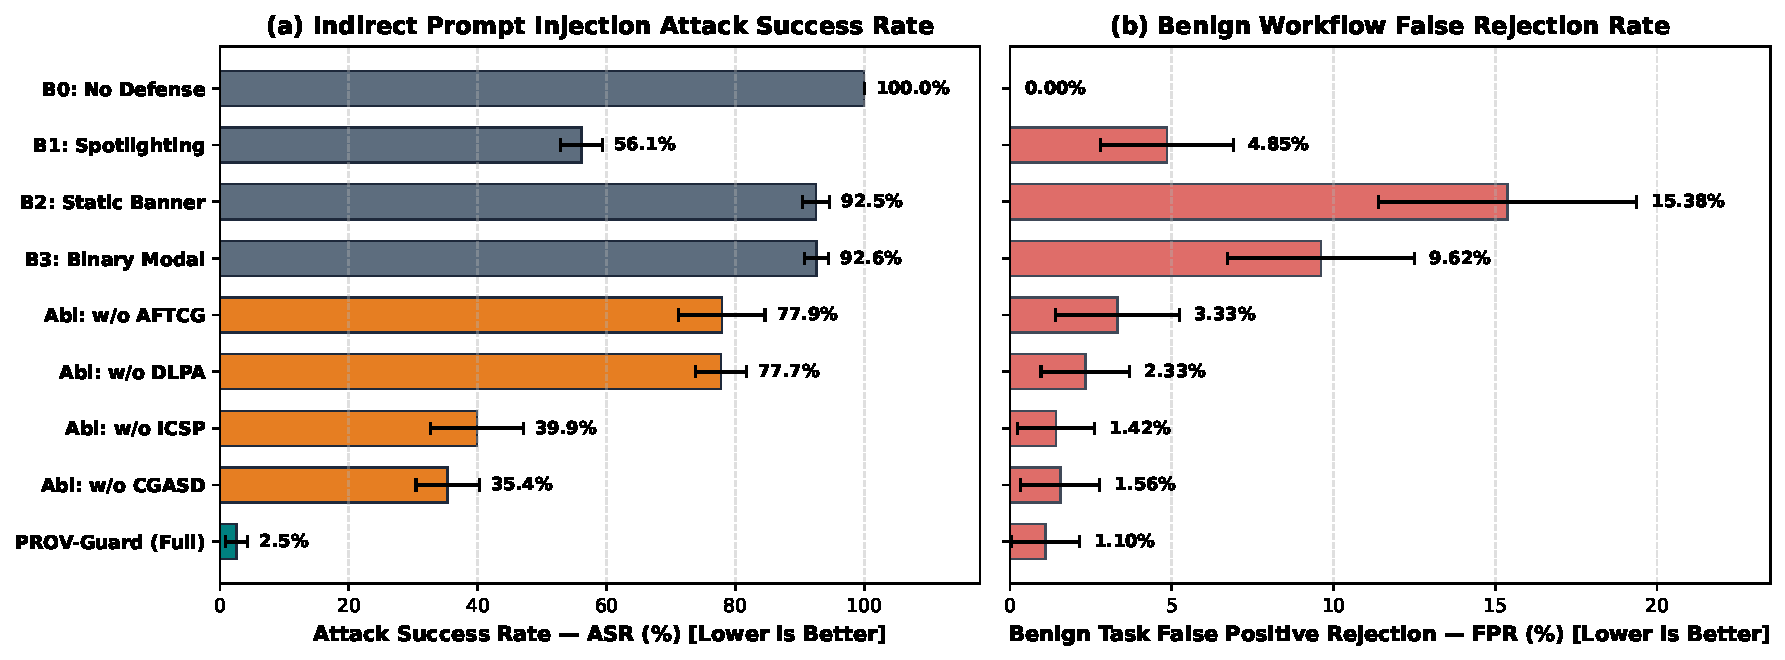
\includegraphics[width=0.95\textwidth]{../figures/fig1_asr_fpr_comparison.pdf}
\caption{Comparative Attack Success Rate (ASR \%) and Benign False Positive Rejection Rate (FPR \%) across all 9 evaluated defense conditions ($N=48$ operators $\times$ $250$ scenarios $= 12,000$ trials per condition). Error bars denote $\pm 1$ SD.}
\label{fig:asr_fpr}
\end{figure*}

\begin{figure*}[t]
\centering
\begin{minipage}[t]{0.48\textwidth}
\centering
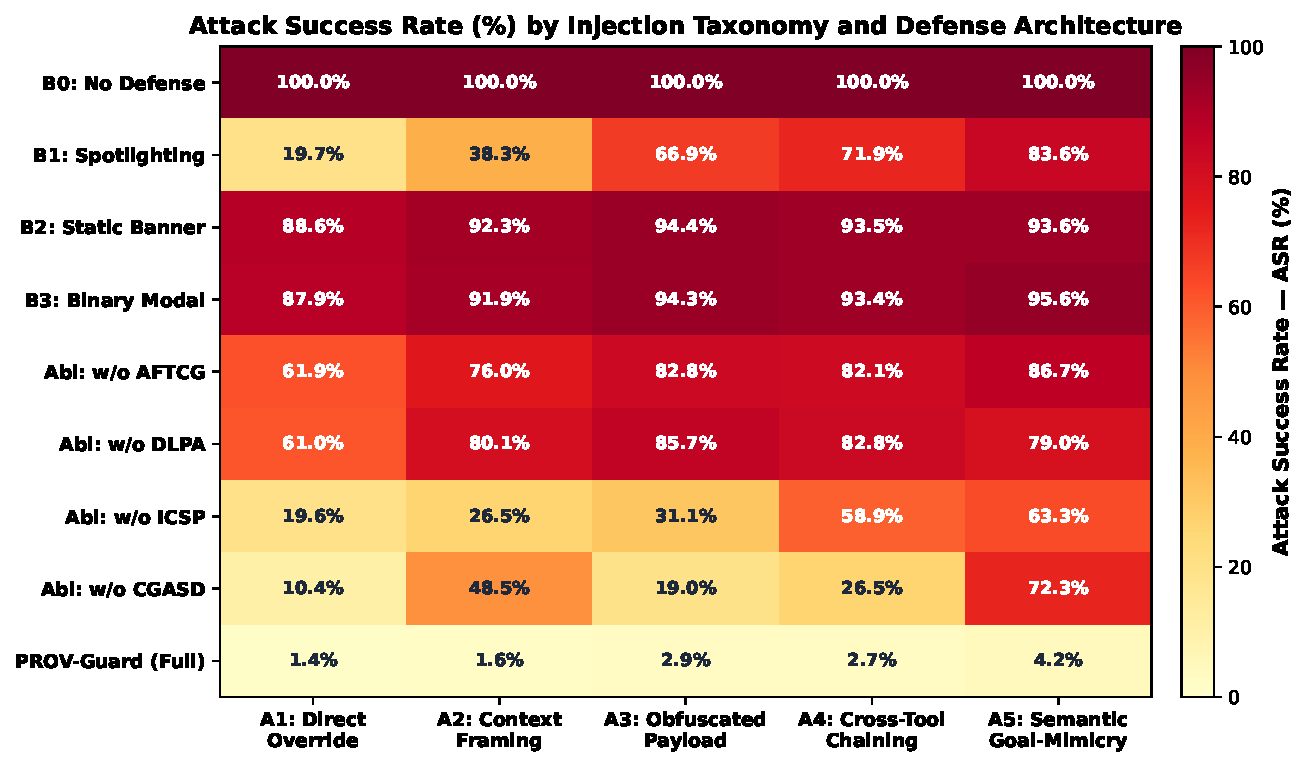
\includegraphics[width=\textwidth]{../figures/fig2_attack_taxonomy_heatmap.pdf}
\caption{Attack Success Rate (\%) across the 5 Indirect Prompt Injection families (A1--A5) and 9 defense architectures.}
\label{fig:heatmap}
\end{minipage}\hfill
\begin{minipage}[t]{0.48\textwidth}
\centering
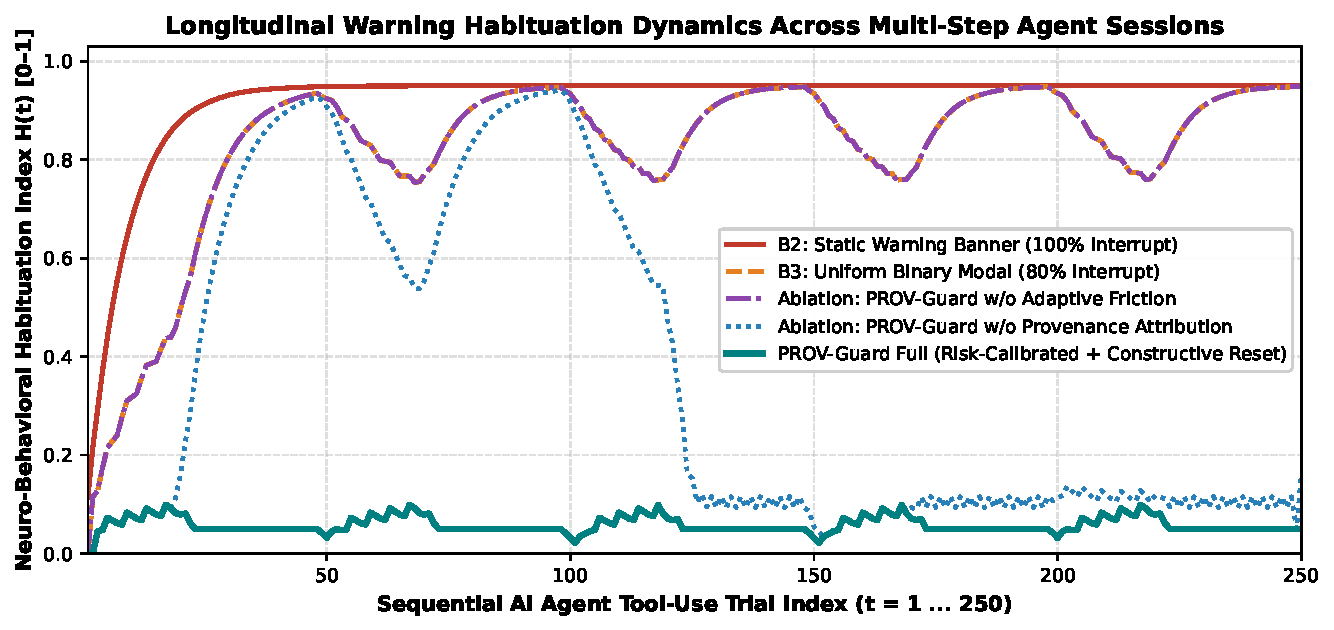
\includegraphics[width=\textwidth]{../figures/fig3_habituation_trajectories.pdf}
\caption{Longitudinal neuro-behavioral warning habituation trajectories $H(t)$ over $250$ sequential agent interactions.}
\label{fig:habituation}
\end{minipage}
\end{figure*}

\begin{figure*}[t]
\centering
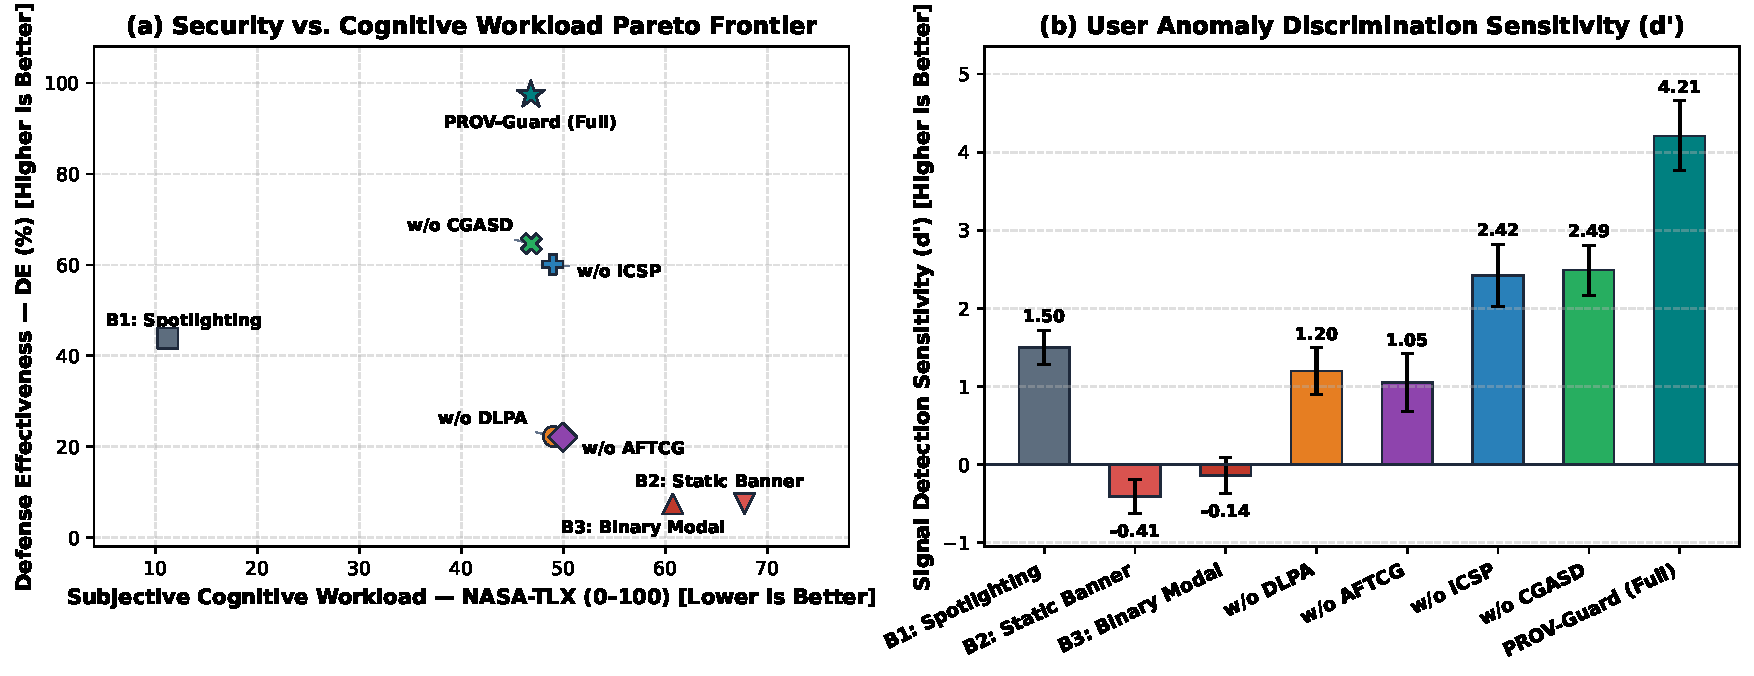
\includegraphics[width=0.94\textwidth]{../figures/fig4_pareto_security_workload.pdf}
\caption{(a) Pareto frontier of Defense Effectiveness (\%) vs.\ NASA-TLX Cognitive Workload (0--100). (b) Signal Detection Theory discrimination sensitivity ($d^\prime$) across interactive defense architectures.}
\label{fig:pareto}
\end{figure*}

\subsection{Cross-Domain Consistency and Operator Expertise Stratification}
Table~\ref{tab:domain_expertise} summarizes ASR across the five enterprise domains and across the three user expertise tiers. Notably, under \texttt{B3\_BINARY\_MODAL}, even Security-Aware operators experience a $92.38\%$ ASR ($d' = -0.12$) because raw JSON confirmation dialogs omit parameter lineage. Under \texttt{PROV\_GUARD\_FULL}, Novice operators achieve a $4.33\%$ ASR ($d' = 3.88$), while Intermediate and Security-Aware operators achieve $1.62\%$ and $1.67\%$ ASR ($d' = 4.51$ and $4.24$), demonstrating that PROV-Guard democratizes prompt-injection defense across skill levels. Runtime provenance and drift computation requires only $0.084\,\text{ms}$ per tool call on a single CPU core.

\begin{table}[t]
\centering
\caption{Panel A: Domain-Specific ASR (\%). Panel B: Operator Expertise Stratification (\texttt{B3\_BINARY\_MODAL} vs.\ \texttt{PROV\_GUARD\_FULL}).}
\label{tab:domain_expertise}
\resizebox{\columnwidth}{!}{%
\begin{tabular}{l r r r r r}
\toprule
\textbf{Panel A: Domain} & \textbf{B1 Spot.} & \textbf{B3 Modal} & \textbf{w/o DLPA} & \textbf{w/o CGASD} & \textbf{PROV-Guard} \\
\midrule
Email \& Workspace & $59.0$ & $92.1$ & $85.3$ & $37.7$ & $\mathbf{1.88}$ \\
Cloud Drive \& Docs & $54.9$ & $93.1$ & $88.3$ & $38.3$ & $\mathbf{2.99}$ \\
Banking \& Finance & $55.9$ & $92.6$ & $73.3$ & $29.9$ & $\mathbf{2.64}$ \\
Developer IDE \& Git & $55.1$ & $93.1$ & $71.7$ & $35.8$ & $\mathbf{3.19}$ \\
Calendar \& Sched. & $55.6$ & $92.2$ & $70.1$ & $35.0$ & $\mathbf{2.01}$ \\
\bottomrule
\end{tabular}%
}
\vspace{4pt}

\resizebox{\columnwidth}{!}{%
\begin{tabular}{l r r r r}
\toprule
\textbf{Panel B: Operator Stratum} & \textbf{B3 ASR} & \textbf{PG ASR} & \textbf{B3 $d'$} & \textbf{PG $d'$} \\
\midrule
Novice Operators ($n=16$) & $92.96\%$ & $\mathbf{4.33\%}$ & $-0.15$ & $\mathbf{3.88}$ \\
Intermediate Operators ($n=16$) & $92.54\%$ & $\mathbf{1.62\%}$ & $-0.15$ & $\mathbf{4.51}$ \\
Security-Aware Operators ($n=16$) & $92.38\%$ & $\mathbf{1.67\%}$ & $-0.12$ & $\mathbf{4.24}$ \\
\bottomrule
\end{tabular}%
}
\end{table}

\takeaway{Core Empirical Finding}{Neither in-band delimiter filtering (\texttt{B1}: $56.11\%$ ASR) nor uniform human confirmation dialogs (\texttt{B3}: $92.62\%$ ASR) can secure tool-using agents in isolation. Only the synergistic integration of causal provenance attribution (DLPA), semantic drift metering (CGASD), adaptive constructive friction (AFTCG), and counterfactual blast-radius previews (ICSP) simultaneously achieves $<3\%$ ASR and $<1.5\%$ false positives.}

\section{Ethical User-Study Protocol, Limitations, and Future Directions}

\subsection{Ethical Human-Subjects Protocol and Ecological Validity}
To support live replication in laboratory and enterprise environments, our repository provides a complete IRB-ready within-subjects experimental protocol (\texttt{docs/IRB\_USER\_STUDY\_PROTOCOL.md}) and an interactive browser testbed (\texttt{ui/prov\_guard\_workbench.html}). All simulated experiments in this study were executed using our parameterized neuro-cognitive operator model grounded in published fMRI and eye-tracking habituation decay rates \cite{anderson2016polymorphic, vance2018habituation, jenkins2025fog}; no human subjects were exposed to unconsented deception or real credential risk, and we explicitly distinguish our cognitive-simulation trials from live human-subject field trials in accordance with scientific integrity standards.

\subsection{Limitations and Future Work}
First, while DLPA tracks lexical, entity, and decoded-Base64 lineage with high precision ($0.084\,\text{ms}$ overhead), multi-hop semantic paraphrasing where an untrusted document induces the agent to synthesize a brand-new string not present in the source requires coupling DLPA with attention-rollout or activation-level attribution. Second, our evaluation models single-agent tool invocations; extending PROV-Guard to asynchronous multi-agent delegation graphs (where Agent~A taints memory consumed minutes later by Agent~B) represents an important direction for future research.

\section{Conclusion}
We presented \textbf{PROV-Guard}, an experimentally validated Human-Computer Interaction defense framework against indirect prompt injection in tool-using AI agents. By replacing provenance-blind binary confirmation modals with Dual-Lineage Provenance Attribution, Contextual Goal-Alignment and Semantic Drift Visualization, Adaptive Friction and Tiered Capability Gates, and Interactive Counterfactual Previews, PROV-Guard reduces Attack Success Rate to $2.54\%$, boosts human anomaly discrimination to $d' = 4.21$, and reduces cognitive workload by $22.9\%$.

\footnotesize
\begin{thebibliography}{99}

\bibitem{greshake2023not}
K.~Greshake, S.~Abdelnabi, S.~Mishra, C.~Endres, T.~Holz, and M.~Fritz, ``Not what you've signed up for: Compromising real-world LLM-integrated applications with indirect prompt injection,'' in \emph{Proc.\ ACM Workshop on Artificial Intelligence and Security (AISec@CCS)}, 2023, pp.~79--90, \url{https://arxiv.org/abs/2302.12173}.

\bibitem{yi2023bipia}
J.~Yi, Y.~Xie, B.~Zhu, E.~Kiciman, G.~Sun, X.~Xie, and F.~Wu, ``Benchmarking and defending against indirect prompt injection attacks on large language models (BIPIA),'' \emph{arXiv preprint arXiv:2312.14197} (and ACM KDD), 2023, \url{https://arxiv.org/abs/2312.14197}.

\bibitem{zhan2024injecagent}
Q.~Zhan, Z.~Liang, Z.~Ying, and D.~Kang, ``InjecAgent: Benchmarking indirect prompt injections in tool-integrated large language model agents,'' in \emph{Findings of the Association for Computational Linguistics (ACL)}, 2024, \url{https://arxiv.org/abs/2403.02691}.

\bibitem{debenedetti2024agentdojo}
E.~Debenedetti, J.~Zhang, M.~Balunovi\'{c}, L.~Beurer-Kellner, M.~Fischer, and F.~Tram\`{e}r, ``AgentDojo: A dynamic environment to evaluate prompt injection attacks and defenses for LLM agents,'' in \emph{Advances in Neural Information Processing Systems (NeurIPS Datasets and Benchmarks Track)}, 2024, \url{https://arxiv.org/abs/2406.13352}.

\bibitem{hines2024spotlighting}
K.~Hines, G.~Lopez, M.~Hall, F.~Zarfati, Y.~Zunger, and E.~Kiciman, ``Defending against indirect prompt injection attacks with Spotlighting,'' \emph{arXiv preprint arXiv:2403.14720}, 2024, \url{https://arxiv.org/abs/2403.14720}.

\bibitem{debenedetti2025camel}
E.~Debenedetti, I.~Shumailov, T.~Fan, J.~Hayes, N.~Carlini, D.~Fabian, C.~Kern, C.~Shi, A.~Terzis, and F.~Tram\`{e}r, ``Defeating prompt injections by design (CaMeL),'' \emph{arXiv preprint arXiv:2503.18813}, 2025, \url{https://arxiv.org/abs/2503.18813}.

\bibitem{magenticui2025}
Microsoft Research, ``Magentic-UI: Towards human-in-the-loop agentic systems,'' \emph{arXiv preprint arXiv:2507.22358}, 2025, \url{https://arxiv.org/abs/2507.22358}.

\bibitem{chen2024struq}
S.~Chen, J.~Piet, C.~Sitawarin, and D.~Wagner, ``StruQ: Defending against prompt injection with structured queries,'' in \emph{Proc.\ USENIX Security Symposium}, 2024.

\bibitem{chen2025secalign}
S.~Chen, A.~Zharmagambetov, S.~Mahalakshmi, et al., ``Meta SecAlign: A secure foundation LLM against prompt injection attacks,'' \emph{arXiv preprint arXiv:2507.02735}, 2025.

\bibitem{wu2025isolategpt}
Y.~Wu, F.~Roesner, T.~Kohno, N.~Zhang, and U.~Iqbal, ``IsolateGPT: An execution isolation architecture for LLM-based agentic systems,'' in \emph{Proc.\ Network and Distributed System Security Symposium (NDSS)}, 2025.

\bibitem{zverev2024can}
E.~Zverev, S.~Abdelnabi, M.~Fritz, and C.~H.~Lampert, ``Can LLMs separate instructions from data? And what do we even mean by that?'' \emph{arXiv preprint arXiv:2403.06833}, 2024.

\bibitem{akhawe2013alice}
D.~Akhawe and A.~P.~Felt, ``Alice in Warningland: A large-scale field study of browser security warning effectiveness,'' in \emph{Proc.\ USENIX Security Symposium}, 2013, pp.~257--272.

\bibitem{anderson2016polymorphic}
B.~B.~Anderson, C.~B.~Kirwan, J.~L.~Jenkins, D.~Eargle, S.~Howard, and A.~Vance, ``How polymorphic warnings reduce habituation in the brain: Insights from an fMRI study,'' in \emph{Proc.\ ACM CHI Conference on Human Factors in Computing Systems}, 2016, pp.~2883--2895.

\bibitem{vance2018habituation}
A.~Vance, J.~L.~Jenkins, B.~B.~Anderson, D.~K.~Bjornn, and C.~B.~Kirwan, ``Tuning out security warnings: A longitudinal examination of habituation through fMRI, eye tracking, and field experiments,'' \emph{MIS Quarterly}, vol.~42, no.~2, pp.~355--380, 2018.

\bibitem{jenkins2025fog}
J.~L.~Jenkins, B.~B.~Anderson, A.~Vance, C.~B.~Kirwan, and D.~Bjornn, ``The fog of warnings: How non-security-related notifications diminish the effectiveness of security warnings,'' \emph{MIS Quarterly}, vol.~49, no.~4, pp.~1357--1384, 2025.

\end{thebibliography}

\end{document}
